\documentclass[UTF8,aspectratio=169,10pt]{ctexbeamer}
\usepackage{etoolbox,tikz,booktabs,amsmath,amssymb,graphicx}
\usetikzlibrary{arrows.meta}
\makeatletter\def\input@path{{template/theme/}}\makeatother
\usetheme{CleanEasy}
\title[漂移扩散方程的数值解]{漂移扩散方程数值实验}
\subtitle{反向随机游走与 Gaussian 宽核直接卷积\\临时实验报告}
\author{}\institute{}\date[]{2026年11月17日}
\hypersetup{pdfauthor={},pdftitle={漂移扩散方程数值实验演示}}
\newcommand{\pic}[1]{\begin{center}\includegraphics[width=.92\linewidth,height=5.1cm,keepaspectratio]{figures/#1.pdf}\end{center}}

% Code blocks: use XeLaTeX and [fragile] on frames containing inline code.
\usepackage{listings,textcomp}
% A local monospace font avoids the theme's legacy Typewriter font fallback.
\newfontfamily\slidecodefont[
  BoldFont=lmmonolt10-bold.otf,
  ItalicFont=lmmono10-italic.otf,
  BoldItalicFont=lmmonolt10-boldoblique.otf,
  Ligatures={NoCommon,TeXOff}
]{lmmono10-regular.otf}
\lstdefinelanguage{RcppArmadillo}[11]{C++}{
  morekeywords=[2]{Rcpp,arma,vec,mat,uvec,umat,sp_mat,subvec,dot,
    linspace,zeros,ones,randu,randn,conv,as,wrap,export,depends}
}
\lstdefinelanguage{RcppEigen}[11]{C++}{
  morekeywords=[2]{Rcpp,Eigen,MatrixXd,VectorXd,MatrixXi,VectorXi,
    SparseMatrix,Triplet,SparseLU,SimplicialLDLT,Map,Ref,Matrix,Vector,
    setFromTriplets,makeCompressed,analyzePattern,factorize,solve,as,wrap}
}
\lstdefinelanguage{PyTorch}[]{Python}{
  morekeywords=[2]{torch,nn,optim,autograd,Tensor,tensor,Module,Linear,
    Sequential,Tanh,ReLU,Parameter,Adam,SGD,grad,backward,zero_grad,
    requires_grad,requires_grad_,no_grad,detach,device,cuda,manual_seed}
}
\lstdefinestyle{slidecode}{
  basicstyle=\slidecodefont\fontsize{7}{9}\selectfont,
  keywordstyle=\color{DarkBlue}\bfseries,
  keywordstyle=[2]\color{MediumBlue}\bfseries,
  commentstyle=\color{green!35!black},
  stringstyle=\color{red!55!black},
  identifierstyle=\color{MediumBlack},
  backgroundcolor=\color{MutedBlack},
  frame=single,
  rulecolor=\color{MediumBlue!50},
  framerule=0.4pt,
  framesep=4pt,
  numbers=left,
  numberstyle=\tiny\color{MediumBlack!65},
  numbersep=6pt,
  xleftmargin=2em,
  xrightmargin=0.5em,
  framexleftmargin=1.5em,
  aboveskip=0.6em,
  belowskip=0.6em,
  columns=fullflexible,
  keepspaces=true,
  tabsize=4,
  breaklines=true,
  breakatwhitespace=false,
  breakautoindent=true,
  breakindent=1em,
  showstringspaces=false,
  showspaces=false,
  showtabs=false,
  upquote=true,
  extendedchars=false,
  captionpos=t,
  abovecaptionskip=0pt,
  belowcaptionskip=4pt,
  resetmargins=false
}
% Optional argument accepts listings options, e.g. title, numbers, firstnumber.
% Language: R, RcppArmadillo, RcppEigen, Python, or PyTorch.
\lstnewenvironment{codeblock}[2][]{
  \lstset{style=slidecode,language=#2,#1}
}{}
% Include a source file (or selected lines) using the same code-block style.
\newcommand{\codefile}[3][]{%
  \lstinputlisting[style=slidecode,language=#2,#1]{#3}%
}

% Usage: code on the left, explanation on the right.
% \begin{frame}[fragile]{代码与说明}
% \begin{columns}[T,onlytextwidth]
%   \begin{column}{0.56\textwidth}
%     \begin{codeblock}[title={R 示例}]{R}
% x <- seq(0, 1, length.out = 101)
% u <- exp(-2 * x) * sin(pi * x)
%     \end{codeblock}
%   \end{column}
%   \begin{column}{0.40\textwidth}
%     \begin{itemize}
%       \item 在这里解释代码。
%     \end{itemize}
%   \end{column}
% \end{columns}
% \end{frame}
% Swap the two column environments to put the code on the right.
% A codeblock outside columns uses the full available width.
% File example (paths are relative to the report directory):
% \codefile[firstline=1,lastline=15]{RcppArmadillo}{../../src/gaussian_convolution.cpp}
% End code-block support.

\begin{document}
\begin{frame}[plain]\titlepage\end{frame}
% Project background sources:
% Black, F. and Scholes, M. (1973), JPE 81(3), 637--654.
% https://doi.org/10.1086/260062
% Jeong, D., Kim, J. and Wee, I.-S. (2009), CKMS 24(4), 617--628.
% https://doi.org/10.4134/CKMS.2009.24.4.617
\section{项目背景}
\begin{frame}{Black--Scholes 模型的用途}
Black--Scholes（B--S）模型用于计算\textbf{期权的理论价格}。
\begin{itemize}
\item 根据当前资产价格、执行价、到期时间、无风险利率和波动率，
      计算期权在当前时刻的价值。
\item 例如欧式看涨期权：持有人可在到期日 $T$ 按执行价 $K$ 购买资产，
      到期收益为 $(S_T-K)_+$，其中 $S_T$ 是到期时的资产价格。
\item 多资产版本可用于篮子期权定价，空间维数对应资产数量。
\end{itemize}
\begin{block}{漂移扩散方程 Drift Diffusion Equation}
对资产价格取对数、用到期剩余时间计时，并消去贴现项后，
B--S 定价方程具有漂移扩散结构。
\begin{equation*}
      \begin{cases}
            u_t(\boldsymbol{x},t) = \boldsymbol{a}\cdot \nabla u(\boldsymbol{x},t) + D\Delta u(\boldsymbol{x},t)\\
            u(\boldsymbol{x},0) = f_0(\boldsymbol{x})
      \end{cases}
\end{equation*}
\end{block}
\vfill
{\scriptsize 来源：\href{https://doi.org/10.1086/260062}{Black \& Scholes (1973)}；
\href{https://doi.org/10.4134/CKMS.2009.24.4.617}{Jeong, Kim \& Wee (2009), pp.\,617--618}。\par}
\end{frame}
% Variable meanings follow Kohn, PDE for Finance, Section 2, pp. 1--2,
% and finmath-lib's MultiAssetBlackScholesModel documentation.
\begin{frame}{漂移扩散方程中各变量的金融含义}
\[
u_\tau=\boldsymbol a\cdot\nabla u+D\Delta u,
\qquad u(\boldsymbol x,0)=f_0(\boldsymbol x).
\]
\begin{description}
\item[$\boldsymbol x$] 对数股价坐标，$x_i=\log S_i$；$S_i$ 为资产价格，$d$ 为资产数量。
\item[$\tau$] 到期剩余时间，$\tau=T-t$；$T$ 为到期时刻，$t$ 为当前时刻。
\item[$u$] 消去贴现项后的期权价值，$u=e^{r\tau}V$；$V$ 为期权当前理论价值。
\item[$\boldsymbol a$] 风险中性下的对数价格漂移，$a_i=r-\sigma_{\rm BS}^2/2$；$r$ 为无风险利率。
\item[$D$] 扩散系数，$D=\sigma_{\rm BS}^2/2$；$\sigma_{\rm BS}$ 为资产收益率波动率。
\item[$f_0$] 到期收益函数，对应剩余期限为零时的初值。
\end{description}
$\nabla u$ 是一阶空间导数向量，$\Delta u=\sum_i u_{x_ix_i}$ 是二阶空间导数之和。
\medskip\par
{\small 上述系数假设无分红、利率与波动率恒定；多资产时还假设独立且波动率相同。
本项目取 $d=1$，用 $t$ 表示此处的 $\tau$，扩散系数也记为 $\sigma^2=D$。}
\vfill
{\scriptsize 来源：\href{https://math.nyu.edu/~kohn/pde.finance/2015/section2.pdf}{Kohn, \emph{PDE for Finance}, \S2, pp.\,1--2}；
\href{https://www.finmath.net/finmath-lib/apidocs/net.finmath.lib/net/finmath/montecarlo/assetderivativevaluation/models/MultiAssetBlackScholesModel.html}{finmath-lib, \emph{MultiAssetBlackScholesModel}}。\par}
\end{frame}
\section{求解算法}

\begin{frame}{四种数值解算法}
      \begin{exampleblock}{解析解}
            \[
            \begin{aligned}
                  u_{\star}(\boldsymbol{x},t)
                  &=\int_{\mathbb R^d}f_0(\boldsymbol{y})\,
                    G_t(\boldsymbol{y}-\boldsymbol{x}-\boldsymbol{a}t)\,d\boldsymbol{y}\\
                  &=(G_t \ast f_0)(\boldsymbol{x} + \boldsymbol{a}t)
            \end{aligned}
            \]
            {\small 其中 $G_t(\boldsymbol{z})=(4\pi Dt)^{-d/2}\exp\bigl(-\|\boldsymbol{z}\|_2^2/(4Dt)\bigr)$
            是 Gaussian 核，$D=\sigma^2$。}
      \end{exampleblock}
      \begin{enumerate}
            \item 反向随机游走（Monte Carlo 采样），\textbf{RcppArmadillo}+\textbf{OpenMP} 并行
            \item Gaussian 宽核直接卷积（类似图像卷积），\textbf{RcppArmadillo}+\textbf{OpenMP} 并行
            \item 显式差分格式，\textbf{RcppEigen} 稀疏矩阵存储与运算
            \item 物理信息神经网络（PINN），\textbf{PyTorch}训练
      \end{enumerate}
      
\end{frame}
\begin{frame}{数值实验}
把空间简化成一维，使用以下方程进行数值实验
\begin{align*}
& u_t = 0.2u_x + 0.05u_{xx}, \quad 0 < x < 1, \quad T = 0.5, \\
& u(0,t)=u(1,t)=0, \qquad f(x)=e^{-2x}\sin(\pi x), \\
& u_{\star}(x,t)=e^{-2x-(0.05\pi^2+0.2)t}\sin(\pi x).
\end{align*}

\begin{itemize}
\item 内部 RMSE 与边界残差分别记录。
\item R 层串行组织实验；C++ OpenMP 使用一、二、四线程。
\item 30 批独立随机重复，性能预热后重复 7 次。
\end{itemize}\end{frame}

\section{反向随机游走}

% Based on idea.md, Section 1; retain the stay-put event p_0 and absorption.
\begin{frame}{三点差分格式与一步反向游走}
取 $x_i=ih$、$t_n=n\tau$、$u_i^n\approx u(x_i,t_n)$，时间前向、空间中心差分：
\begin{columns}[c,onlytextwidth]
\begin{column}{0.61\textwidth}
\[
\frac{u_i^{n+1}-u_i^n}{\tau}
=a\frac{u_{i+1}^n-u_{i-1}^n}{2h}
 +D\frac{u_{i+1}^n-2u_i^n+u_{i-1}^n}{h^2}.
\]
\[
\boxed{u_i^{n+1}=p_-u_{i-1}^n+p_0u_i^n+p_+u_{i+1}^n}
\]
\[
\begin{aligned}
p_\pm&=\frac{D\tau}{h^2}\pm\frac{a\tau}{2h},\\
p_0&=1-\frac{2D\tau}{h^2}.
\end{aligned}
\]
当 $\dfrac{D\tau}{h^2}\le\dfrac12$、$|a|h\le2D$ 时，
$p_-,p_0,p_+\ge0$ 且和为 $1$，可作为转移概率。
\end{column}
\begin{column}{0.36\textwidth}
\centering
{\scriptsize\textbf{差分推进：第 $n$ 层计算第 $n+1$ 层}}\par
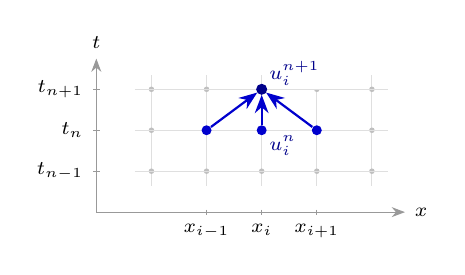
\begin{tikzpicture}[x=.70cm,y=.52cm,>=Stealth,font=\scriptsize]
  % Axes and the regular space-time mesh.
  \draw[->,gray!80] (0,0)--(5.6,0) node[right,text=black] {$x$};
  \draw[->,gray!80] (0,0)--(0,3.75) node[above,text=black] {$t$};
  \foreach \xx in {1,2,3,4,5} {
    \draw[gray!25] (\xx,.65)--(\xx,3.35);
    \foreach \yy in {1,2,3} {\fill[gray!50] (\xx,\yy) circle (1pt);}
  }
  \foreach \yy in {1,2,3} {\draw[gray!25] (.7,\yy)--(5.3,\yy);}
  \foreach \xx/\lab in {2/{i-1},3/{i},4/{i+1}} {
    \draw[gray!80] (\xx,.06)--(\xx,-.06);
    \node[below] at (\xx,-.06) {$x_{\lab}$};
  }
  \foreach \yy/\lab in {1/{n-1},2/{n},3/{n+1}} {
    \draw[gray!80] (-.06,\yy)--(.06,\yy);
    \node[left] at (-.06,\yy) {$t_{\lab}$};
  }
  % FTCS uses three values on row n to update the centre on row n+1.
  \foreach \xx in {2,3,4} {
    \draw[->,MediumBlue,thick,shorten >=2pt,shorten <=2pt] (\xx,2)--(3,3);
    \fill[MediumBlue] (\xx,2) circle (1.8pt);
  }
  \fill[DarkBlue] (3,3) circle (2pt);
  \node[below right,text=DarkBlue,fill=white,inner sep=1pt]
    at (3.08,1.94) {$u_i^n$};
  \node[above right,text=DarkBlue,fill=white,inner sep=1pt]
    at (3.08,3) {$u_i^{n+1}$};
\end{tikzpicture}
\par\smallskip
{\scriptsize\textbf{随机回溯：第 $n+1$ 层返回第 $n$ 层}}\par
\begin{tikzpicture}[x=.85cm,y=.85cm,>=Stealth,font=\scriptsize]
  \draw[gray!35,dashed] (-2,1.5)--(2,1.5);
  \draw[gray!35,dashed] (-2,0)--(2,0);
  \node[above,text=DarkBlue] at (0,1.55) {$u_i^{n+1}$};
  \fill[DarkBlue] (0,1.5) circle (2.2pt);
  \draw[->,thick,MediumBlue,shorten >=3pt,shorten <=3pt]
    (0,1.5)--(-1.6,0) node[midway,above left] {$p_-$};
  \draw[->,thick,MediumBlue,shorten >=3pt,shorten <=3pt]
    (0,1.5)--(0,0) node[midway,right] {$p_0$};
  \draw[->,thick,MediumBlue,shorten >=3pt,shorten <=3pt]
    (0,1.5)--(1.6,0) node[midway,above right] {$p_+$};
  \foreach \xx/\lab in {-1.6/{i-1},0/{i},1.6/{i+1}} {
    \fill[MediumBlue] (\xx,0) circle (2pt);
    \node[below] at (\xx,-.03) {$u_{\lab}^n$};
  }
  \node[right,font=\scriptsize] at (2,1.5) {$t_{n+1}$};
  \node[right,font=\scriptsize] at (2,0) {$t_n$};
  \node[font=\scriptsize,align=center] at (0,-.76)
    {时间回退 $\tau$，空间移动 $-h$、$0$ 或 $+h$};
\end{tikzpicture}
\end{column}
\end{columns}
\end{frame}

\begin{frame}{反向随机游走的期望表示}
由一步递推式
\[
u_i^{n+1}=p_-u_{i-1}^n+p_0u_i^n+p_+u_{i+1}^n,
\]
逐层回溯至 $t=0$，并代入初值 $u_i^0=f_0(x_i)$，可得
\[
\boxed{u_i^n=\mathbb E\!\left[f_0(X_n)\mid X_0=x_i\right]}.
\]
其中，$X_k$ 表示回溯 $k$ 步后的位置。在首次触边前，
\[
X_k=x_i+h\sum_{j=1}^{k}\xi_j,
\qquad \xi_1,\xi_2,\ldots\ \text{独立同分布},
\]
\[
\mathbb P(\xi_j=-1)=p_-,\qquad
\mathbb P(\xi_j=0)=p_0,\qquad
\mathbb P(\xi_j=+1)=p_+.
\]
\begin{block}{零边界对应吸收}
路径触及 $0$ 或 $1$ 后停留在该边界。
由于 $f_0(0)=f_0(1)=0$，触边路径的收益为零。
\end{block}
\end{frame}

\begin{frame}{Monte Carlo：用路径平均估计期望}
独立模拟 $M$ 条反向随机游走路径，记第 $m$ 条路径的终点为 $X_n^{(m)}$。
\medskip
\begin{columns}[T,onlytextwidth]
\begin{column}{0.53\textwidth}
\textbf{以终点初值的样本均值估计 $u_i^n$}
\[
\begin{aligned}
Y_m&=f_0(X_n^{(m)}),\\
\widehat u_i^n&=\textstyle\frac1M\sum_{m=1}^{M}Y_m.
\end{aligned}
\]
\begin{itemize}
\item 从 $X_0=x_i$ 按三个概率回溯至初始时刻。
\item 触边计 $0$，仍对\textbf{全部 $M$ 条路径}取平均。
\end{itemize}
{\small 期望严格等于差分解，有限样本平均另有抽样误差。}
\end{column}
\begin{column}{0.44\textwidth}
\centering
% Static placeholder: compilation does not require animation packages or files.
\fbox{\parbox[c][3.8cm][c]{0.94\linewidth}{\centering
  \color{MediumBlack}反向随机游走动画\\[0.8em]
  \small 预留展示区域}}
\par\smallskip
{\scriptsize 回溯至 $t=0$，触边立即吸收。}
\end{column}
\end{columns}
\end{frame}

% Existing serial E0 experiment, not a new run.
% Source: scripts/01_tests.R; results/tests/e0_tests.csv.
\begin{frame}{反向随机游走的小规模正确性测试}
\begin{columns}[T,onlytextwidth]
\begin{column}{0.48\textwidth}
\begin{block}{测试设置与参照}
\begin{itemize}
\item $N=n=8$，查询 $x_1=1/8$，$T=0.5$。
\item 串行独立重复 $10$ 批，每批 $M=4096$ 条路径。
\item 以同一差分格式的离散期望为参照，检验抽样误差。
\end{itemize}
\end{block}
\end{column}
\begin{column}{0.48\textwidth}
\begin{block}{抽样误差检验}
\[
z=\frac{|\overline{\widehat u}-u_{\rm disc}|}
        {\sqrt{\operatorname{Var}(Y)/(10M)}}
\]
\[
\boxed{z=0.0502879<4\quad\text{通过}}
\]
{\footnotesize 分母为 $10$ 批平均估计的理论标准误。}
\end{block}
\end{column}
\end{columns}
\medskip
\begin{exampleblock}{R 与 Rcpp 的实现一致性也通过}
同随机流、$256$ 条路径下，返回统计量的最大差异小于 $10^{-12}$。
\end{exampleblock}
\vfill
{\scriptsize 测试脚本：\texttt{scripts/01\_tests.R}；
已记录结果：\texttt{results/tests/e0\_tests.csv}。\par}
\end{frame}

% E1 and E2 reuse the recorded 30-batch results in report.tex, Section 3.
\begin{frame}{模拟游走次数对精度的影响（E1）}
\small
$(N,n)=(8,8),(16,32)$，查询 $x=1/8$，$T=0.5$；\\
$M=256,1024,4096,16384$，每个配置独立重复 $30$ 批。
\begin{center}
\includegraphics[width=.98\linewidth,height=4.0cm,keepaspectratio]{figures/mc_error.pdf}
\end{center}
\begin{itemize}
\item \textbf{增加 $M$ 降低抽样误差：}相对差分格式的 RMSE 总体按 $M^{-1/2}$ 下降，有限批次的观测会有波动。
\item \textbf{固定网格仍有误差限制：}$(8,8)$ 的差分格式误差为 $2.39\times10^{-3}$；
      $M=16384$ 时总 RMSE 为 $2.67\times10^{-3}$，已接近这一水平。
\end{itemize}
\end{frame}

\begin{frame}{网格大小对精度的影响（E2）}
\small
固定 $M=4096$，查询 $x=1/8$，每个配置独立重复 $30$ 批；\\
$(N,n)=(8,8),(16,32),(32,128)$，$h=1/N$，保持 $D\tau/h^2=0.2$。
\begin{center}
\includegraphics[width=.98\linewidth,height=3.8cm,keepaspectratio]{figures/mc_grid.pdf}
\end{center}
\begin{itemize}
\item \textbf{$h$ 越小，差分格式误差越小：}由 $2.39\times10^{-3}$ 降至
      $5.75\times10^{-4}$、$1.42\times10^{-4}$。
\item \textbf{随机误差占优时，观测 RMSE 不一定随 $h$ 减小而减小：}
      固定 $M$ 下的抽样波动可掩盖网格改善；总 RMSE 依次为
      $3.77,\,2.71,\,3.22\; (\times10^{-3})$。
\end{itemize}
\end{frame}

% New measured cost experiments: results/walk-cost-20261118/.
% Reproduce with scripts/06_benchmark_walk_cost.R and scripts/07_plot_walk_cost.py.
\begin{frame}{固定线程数：时间与空间网格的开销}
\small
固定 $p=2$、$M=16384$，仅查询 $x=1/2$，$T=0.5$；分别改变 $n$ 与 $N$。\\
计完整求解调用，排除编译、输入准备和预热；$9$ 轮取中位数，误差棒为四分位区间。
\begin{center}
\includegraphics[width=.98\linewidth,height=3.8cm,keepaspectratio]{figures/walk_cost_grid.pdf}
\end{center}
\begin{itemize}
\item \textbf{固定 $N$：}计算量随时间步数 $n$ 为 $O(n)$。
\item \textbf{固定 $n$：}游走主体对 $N$ 为 $O(1)$，另有 $O(N)$ 的输入校验开销。
\end{itemize}
{\footnotesize 时间步数 $n$ 需与空间网格匹配、满足差分格式的稳定性要求，不能随意选取。}
\end{frame}

\begin{frame}{固定求解任务：串行与并行加速}
\small
$(N,n)=(64,512)$，$M=65536$，单点 $x=1/2$；i7-11800H，$8$ 个物理核。\\
串行版关闭 OpenMP；各版本共用算法、随机数流及 R 包装，输出与实际步数一致。
\begin{center}
\includegraphics[width=.98\linewidth,height=3.8cm,keepaspectratio]{figures/walk_cost_parallel.pdf}
\end{center}
\begin{itemize}
\item $S_p=T_{\rm serial}/T_p$：串行 $311.6\,\mathrm{ms}$；
      $2/4/8$ 线程分别为 $154.1/80.9/50.4\,\mathrm{ms}$，加速 $2.02/3.85/6.18$ 倍。
\item $8$ 线程效率约 $77\%$；增加线程仍有收益，但未达到理想线性加速。
      各配置预热后重复 $9$ 轮，以耗时中位数计算加速比。
\end{itemize}
\end{frame}

\begin{frame}{误差、适用范围与计算瓶颈}
\small
\[
\mathbb E\bigl[(\widehat u-u)^2\bigr]
=\underbrace{(u_{\rm disc}-u)^2}_{\text{差分格式误差平方}}
+\underbrace{\operatorname{Var}(Y)/M}_{\text{抽样方差}}.
\]
\begin{columns}[T,onlytextwidth]
\begin{column}{0.48\textwidth}
\textbf{精度与计算代价}
\begin{itemize}
\item 固定网格下，随机标准误减半需要约 $4$ 倍路径数；增加 $M$ 不能消除差分格式误差。
\item 增加时间步数会延长游走；每增加一个查询点，都需要重新模拟一批路径。
\item 因而更适合\textbf{少量查询点、适中精度、可并行的大批路径}。
      一维全网格高精度求解时，逐点重复抽样的成本较高。
\end{itemize}
\end{column}
\begin{column}{0.48\textwidth}
\textbf{本实现的主要限制}
\begin{itemize}
\item 每条路径逐步生成随机数、判断移动与吸收；路径内部的步骤有先后依赖。
\item 路径间可并行，但实际长度不同；本实现每查询点固定 $16$ 个任务块。
\item R 打包与归约、线程调度仍有开销；增加线程不能降低 $M,n$ 所决定的总工作量。
\end{itemize}
\end{column}
\end{columns}
\medskip
{\footnotesize 上述效率来自本机单点任务；查询位置影响吸收概率与实际步数，不能把该加速比直接推广到所有任务。}
\end{frame}

\begin{frame}{反向随机游走}
\[
p_\pm=D\tau/h^2\pm a\tau/(2h),\qquad p_0=1-2D\tau/h^2
\]
\[
Y=f(X_n)\mathbf1_{\{\text{未触边}\}},\qquad \widehat u=M^{-1}\sum Y_k
\]
\begin{itemize}
\item 从查询点出发，逐步吸收，触边贡献为零。
\item 分母包含所有路径，每查询点固定 16 个逻辑块。
\item OpenMP 分配路径块，私有随机流，按块序归约。
\end{itemize}
\begin{exampleblock}{正确性}23 项一线程 E0 测试通过，包含同流、吸收、手算宽核及解析核验；另通过 7 项 OpenMP 集成核验。\end{exampleblock}
\end{frame}
\begin{frame}{正确零边界的 Gaussian 直接卷积}
\[
v=e^{\beta x+\gamma t}u,\quad g=e^{\beta x}f,\quad v_t=Dv_{xx}
\]
\[
u(x,T)=e^{-\beta x-\gamma T}\int_{\mathbb R}G_T(z)\widetilde g(x-z)\,dz
\]
\begin{enumerate}
\item 对变换后的 $g$ 作两端奇延拓，形成周期 2 的辅助输入。
\item Gaussian 宽窗口直接内积，输入只读、输出独立。
\item 乘指数因子变回原解，记录端点置零前残差。
\end{enumerate}
\begin{block}{实现}OpenMP 按输出点并行；RcppArmadillo 的 \texttt{subvec} 与 \texttt{dot} 完成每个窗口。\end{block}
\end{frame}
\begin{frame}{卷积核大小的选择}
\[
s_T=\sqrt{2DT},\quad K=\lceil c s_T/h\rceil,\quad W=2K+1
\]
\begin{itemize}
\item $c$ 决定物理覆盖，$h$ 将范围换算成数组长度。
\item 左右对称加中心点，使奇延拓边界贡献成对抵消。
\item $N=512,c=3$ 时 $K=344,W=689$。
\item 截断后不重新归一化。更宽的核需要更多计算。
\end{itemize}
\begin{exampleblock}{实验控制}核大小实验固定网格；网格实验固定物理覆盖。\end{exampleblock}
\end{frame}
\begin{frame}{核大小与精度、成本}
\pic{kernel}
\small $W=231$ 到 $917$，RMSE 从 $3.84\times10^{-2}$ 降至 $1.62\times10^{-5}$；$W=1375$ 为 $1.90\times10^{-10}$。
\end{frame}
\begin{frame}{宽核下的网格求积误差}
\pic{grid}
\small 多项式初值 $e^{-2x}x(1-x)$，$c=8$；本组观测阶 4.01--4.03，不推广为任意初值的统一结论。
\end{frame}
\begin{frame}{并行任务与计时范围}
\begin{itemize}
\item R 串行调度；C++ 用 OpenMP 并行循环，BLAS 单线程。
\item MC 私有 RNG、固定块序归约；卷积共享完整奇延拓。
\item 串并行预测与 MC 计数一致，预热后重复计时 7 次。
\item $t_{\rm solve}$ 含 R/C++ 调用、fork/join、计算与归约。
\end{itemize}
\[
t_{\rm new}=t_{\rm input}+t_{\rm solve},\qquad
t_{\rm once}=t_{\rm new}+t_{\rm OpenMP\ init}
\]
\begin{block}{首次请求及核验：单次 R 包装调用观测}两线程 1.001 ms，四线程 0.534 ms，含检查且可复用既有线程。$t_{\rm once}$ 不是新 R 进程冷启动；随机流分配、编译、预热与真值核验不计时。\end{block}
\end{frame}
\begin{frame}{并行收益取决于任务规模}
\pic{speedup}
\small 本次大任务四线程：MC \textbf{3.49 倍}，卷积 \textbf{3.66 倍}。个别 $S_p$ 略高于 $p$ 可由有限次数计时、频率及调度波动引起，不构成超线性加速保证。
\end{frame}
\begin{frame}{共同查询任务的精度与成本}
\pic{cost}
\small 共同 8 点、两线程。MC $M=16384$ 与卷积 $c=2$ 的新输入成本比为 \textbf{69.6}，加首次请求核验观测后为 16.0；结论限于本次问题。
\end{frame}
\end{document}
